\appendix

\chapter{Meeting Minutes and Working Records}

\section{Recovered Checkpoint (15/03/2026)}

No formal implementation meeting minutes were archived in the local workspace for the first prototype checkpoint. To avoid inventing details, the following recovered checkpoint summary was compiled from dated artifacts that are present in the repository: the architecture constraints note, the first-pass script plan, and the prototype screenshots created on 15/03/2026.

\begin{itemize}
\item \textbf{Record type:} recovered implementation checkpoint compiled from local artifacts rather than formal minutes.
\item \textbf{Date:} 15/03/2026.
\item \textbf{Attendance:} exact attendance was not archived in the local workspace and should be replaced with confirmed team attendance if chat or calendar records are available.
\item \textbf{Sources used:} \path{demo_architecture_constraints.md}, \path{demo_first_pass_scripts.md}, and prototype screenshots timestamped on 15/03/2026.
\item \textbf{Main focus:} reduce the original game concept to one battle scene, four starter cards, a readable control loop, and a minimum set of scripts that can compile and run inside the existing Unity project.
\item \textbf{Confirmed decisions:} single-battle scope, shared unit controller, deterministic enemy response, explicit card types, button-driven card interaction, and no campaign or deckbuilding systems in WR2.
\item \textbf{Follow-up actions:} finish the first gameplay skeleton, refresh UML diagrams to match implementation, and gather prototype evidence for WR2.
\end{itemize}

\section{WR1 Kickoff and Alignment Meetings}

The following two short records are retained because WR2 directly inherits the role allocation and initial scope decisions set during WR1 preparation.

\subsection{Meeting 1 (17/03/2026)}

\textbf{Time}

17/03/2026

\textbf{Attendance}

\begin{itemize}
\item Guangjun HU
\item Hongshuo HU
\item Zehan CHEN
\end{itemize}

\textbf{Context}

Team members shared their initial game ideas and implementation interests, then narrowed the coursework direction to a tactical card battle demo. The meeting also established the first division of labour and the expected delivery dates for WR1 inputs.

\textbf{Decisions}

Project direction was confirmed as \projectname{}, the initial role allocation was agreed, and individual task expectations were set for the first weekly cycle.

\textbf{Owner}

Guangjun HU, Hongshuo HU, and Zehan CHEN, with follow-up input from Cheng YE.

\textbf{Deadline}

18/03/2026 to 19/03/2026 for the first WR1 materials and task allocation outputs.

\textbf{Follow-up}

These decisions fed directly into the project direction, division of labour, and requirement sections of WR1.

\subsection{Meeting 2 (18/03/2026)}

\textbf{Time}

18/03/2026

\textbf{Attendance}

\begin{itemize}
\item Guangjun HU
\item Cheng YE
\end{itemize}

\textbf{Context}

The team aligned the current requirement scope around a tactical card battle demo, confirmed UML-related responsibilities, and standardised a lightweight meeting-minutes format so later weekly records would be more traceable than the earliest prototype cycle.

\textbf{Decisions}

The current WR1 scope was aligned around a tactical card battle demo, UML diagram production was assigned, and a unified meeting-minutes format was defined for subsequent meetings.

\textbf{Owner}

Guangjun HU and Cheng YE, with follow-up support from the whole team.

\textbf{Deadline}

19/03/2026 for WR1 alignment, followed by use of the agreed meeting-minutes format in later weekly cycles.

\textbf{Follow-up}

These outcomes were reflected in WR1 requirements, UML diagrams, and the documentation process used by later reports.

\section{WR2 Evidence Freeze Note}

The WR2 documentation pack uses an evidence freeze line of \textbf{02/04/2026 12:00}. This freeze is recorded in \path{wr2-snapshot-freeze-2026-04-02.md}. After that point, only changes that materially improve submission quality should be described in WR2. New features developed later should be documented in WR3 or the final report instead of being backfilled into this report.

\section{Supporting Record Index}

The local record structure created during WR2 is summarised below and stored under \texttt{doc/src/project-records}.

\begin{itemize}
\item \path{wr2-asset-register.md}: reusable evidence list, missing items, suggested owners, and due times.
\item \path{process/canonical-repo-evidence-2026-04-02.md}: canonical repository evidence note, historical discovery summary, and the current recommendation for using merged GitHub history as repo-workflow evidence.
\item \path{process/task-board-evidence-2026-04-02.md}: task-board evidence note, discovery summary, and import checklist.
\item \path{process/project-implementation-timeline-gantt.drawio}: draw.io source for the coursework timeline Gantt chart used in the WR2 reflections section.
\item \path{process/task-board/retrospective-wr2-closeout-board.png}: retrospective coordination board reconstructed from the recorded TODO list and merged PR history for explanation only.
\item \path{process/discovery/README.md}: command-level discovery artifacts explaining what was checked from this workspace.
\item \path{meetings/meeting-minutes-template.md}: lightweight meeting template for future weekly records.
\item \path{meetings/meeting-2026-03-17-wr1-kickoff.md}: preserved WR1 kickoff note covering project direction and first role allocation.
\item \path{meetings/meeting-2026-03-18-wr1-alignment.md}: preserved WR1 alignment note covering scope confirmation and meeting-template setup.
\item \path{meetings/implementation-checkpoint-recovered-2026-03-15.md}: transparent recovered note based on local artifacts.
\item \path{decisions/wr2-implementation-decisions.md}: decision log extracted from the current implementation direction.
\item \path{collaboration-history-2026-04-02.md}: concise explanation of the move from early WeChat/Overleaf coordination to the current GitHub PR workflow.
\item \path{validation/wr2-heuristic-walkthrough-2026-04-01.md}: internal WR2 walkthrough and findings.
\item \path{testing/prototype-accuracy-editmode-run-2026-04-02.md}: EditMode verification note for the battle-end accuracy fix.
\item \path{testing/wr3-prep-log-2026-04-01.md}: initial test and bug tracking preparation note for the next report cycle.
\end{itemize}

These records are intentionally lightweight. Their purpose is to stop evidence loss between WR2 and WR3, not to pretend that the record-keeping process was already complete earlier in the prototype cycle.

\section{Retrospective Coordination Board}

\begin{figure}[H]
\centering
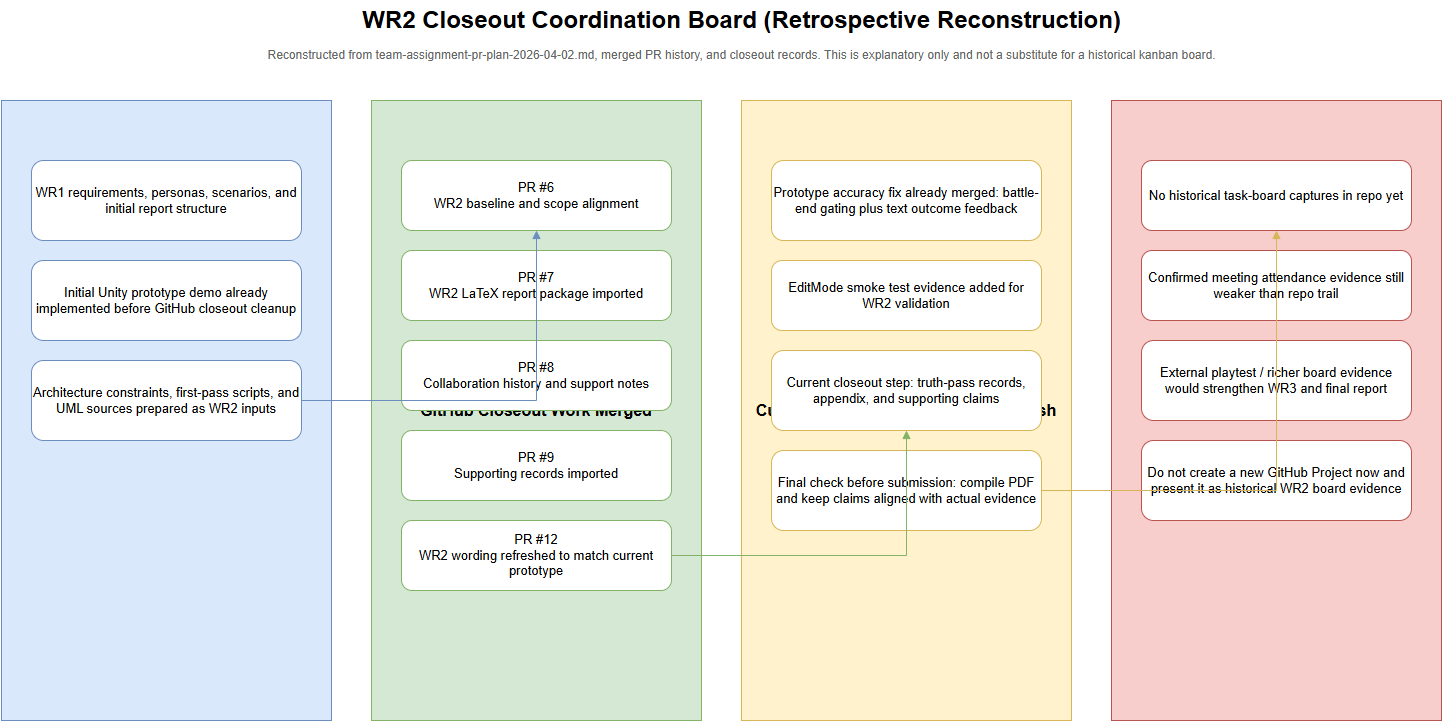
\includegraphics[width=\textwidth]{../project-records/process/task-board/retrospective-wr2-closeout-board.png}
\caption{Retrospective reconstruction of the WR2 closeout board, based on recorded TODO lists and merged GitHub PR history}
\label{fig:wr2-retrospective-board}
\end{figure}

Figure~\ref{fig:wr2-retrospective-board} is included as an explanatory reconstruction because no historical task-board capture survives in the repository. It helps summarise how the closeout work was grouped after the move to GitHub PR workflow, but it is not claimed as original planning-board evidence from the active implementation period.
